% ================= 6. ELECTRONICS =================
\section{Electronics}
\label{sec:electrical}

This section is presented at the level of the decisions that shape the
electrical architecture: what the components are, how the whole system loop
fits together, how power is distributed, how the buses are routed and
terminated, and how the assembly is made safe to power on. The sheet-level
schematics, the connector and pin tables, the harness drawings and the
perfboard layout are collected in Appendix~\ref{app:electrical}, for the same
reason the CAD detail is separated from the mechanical rationale of
Section~\ref{sec:cad} --- a connector re-pin should not require an edit here.
The acceptance criteria and checks run against this architecture during
bring-up (CAN-bus termination, rail voltages, sensor and driver calibration)
are stated with the rest of the verification work in
Section~\ref{sec:verification}, not repeated here.

\subsection{System Architecture}
\label{sec:architecture}

Figure~\ref{fig:system_loop} shows the closed control loop that ties the four
subsystems together. The Teensy~4.1 runs estimation and control at
\qty{1}{\kilo\hertz} and issues torque commands over CAN-FD to three moteus-n1
drivers, each closing a \qty{30}{\kilo\hertz} field-oriented current loop on its
MN4006 motor. The resulting reaction torque acts on the cube body; the body's
attitude is sensed by the BMI270 IMU and the rotor angle by the MA600 absolute
encoder, closing the loop back to the controller. The two loops run at different
rates by design: the fast current loop is delegated entirely to the drivers, so
the flight controller need only meet the \qty{1}{\milli\second} outer-loop
deadline of Section~\ref{sec:control_algorithms}.

\begin{figure}[htbp]
\centering
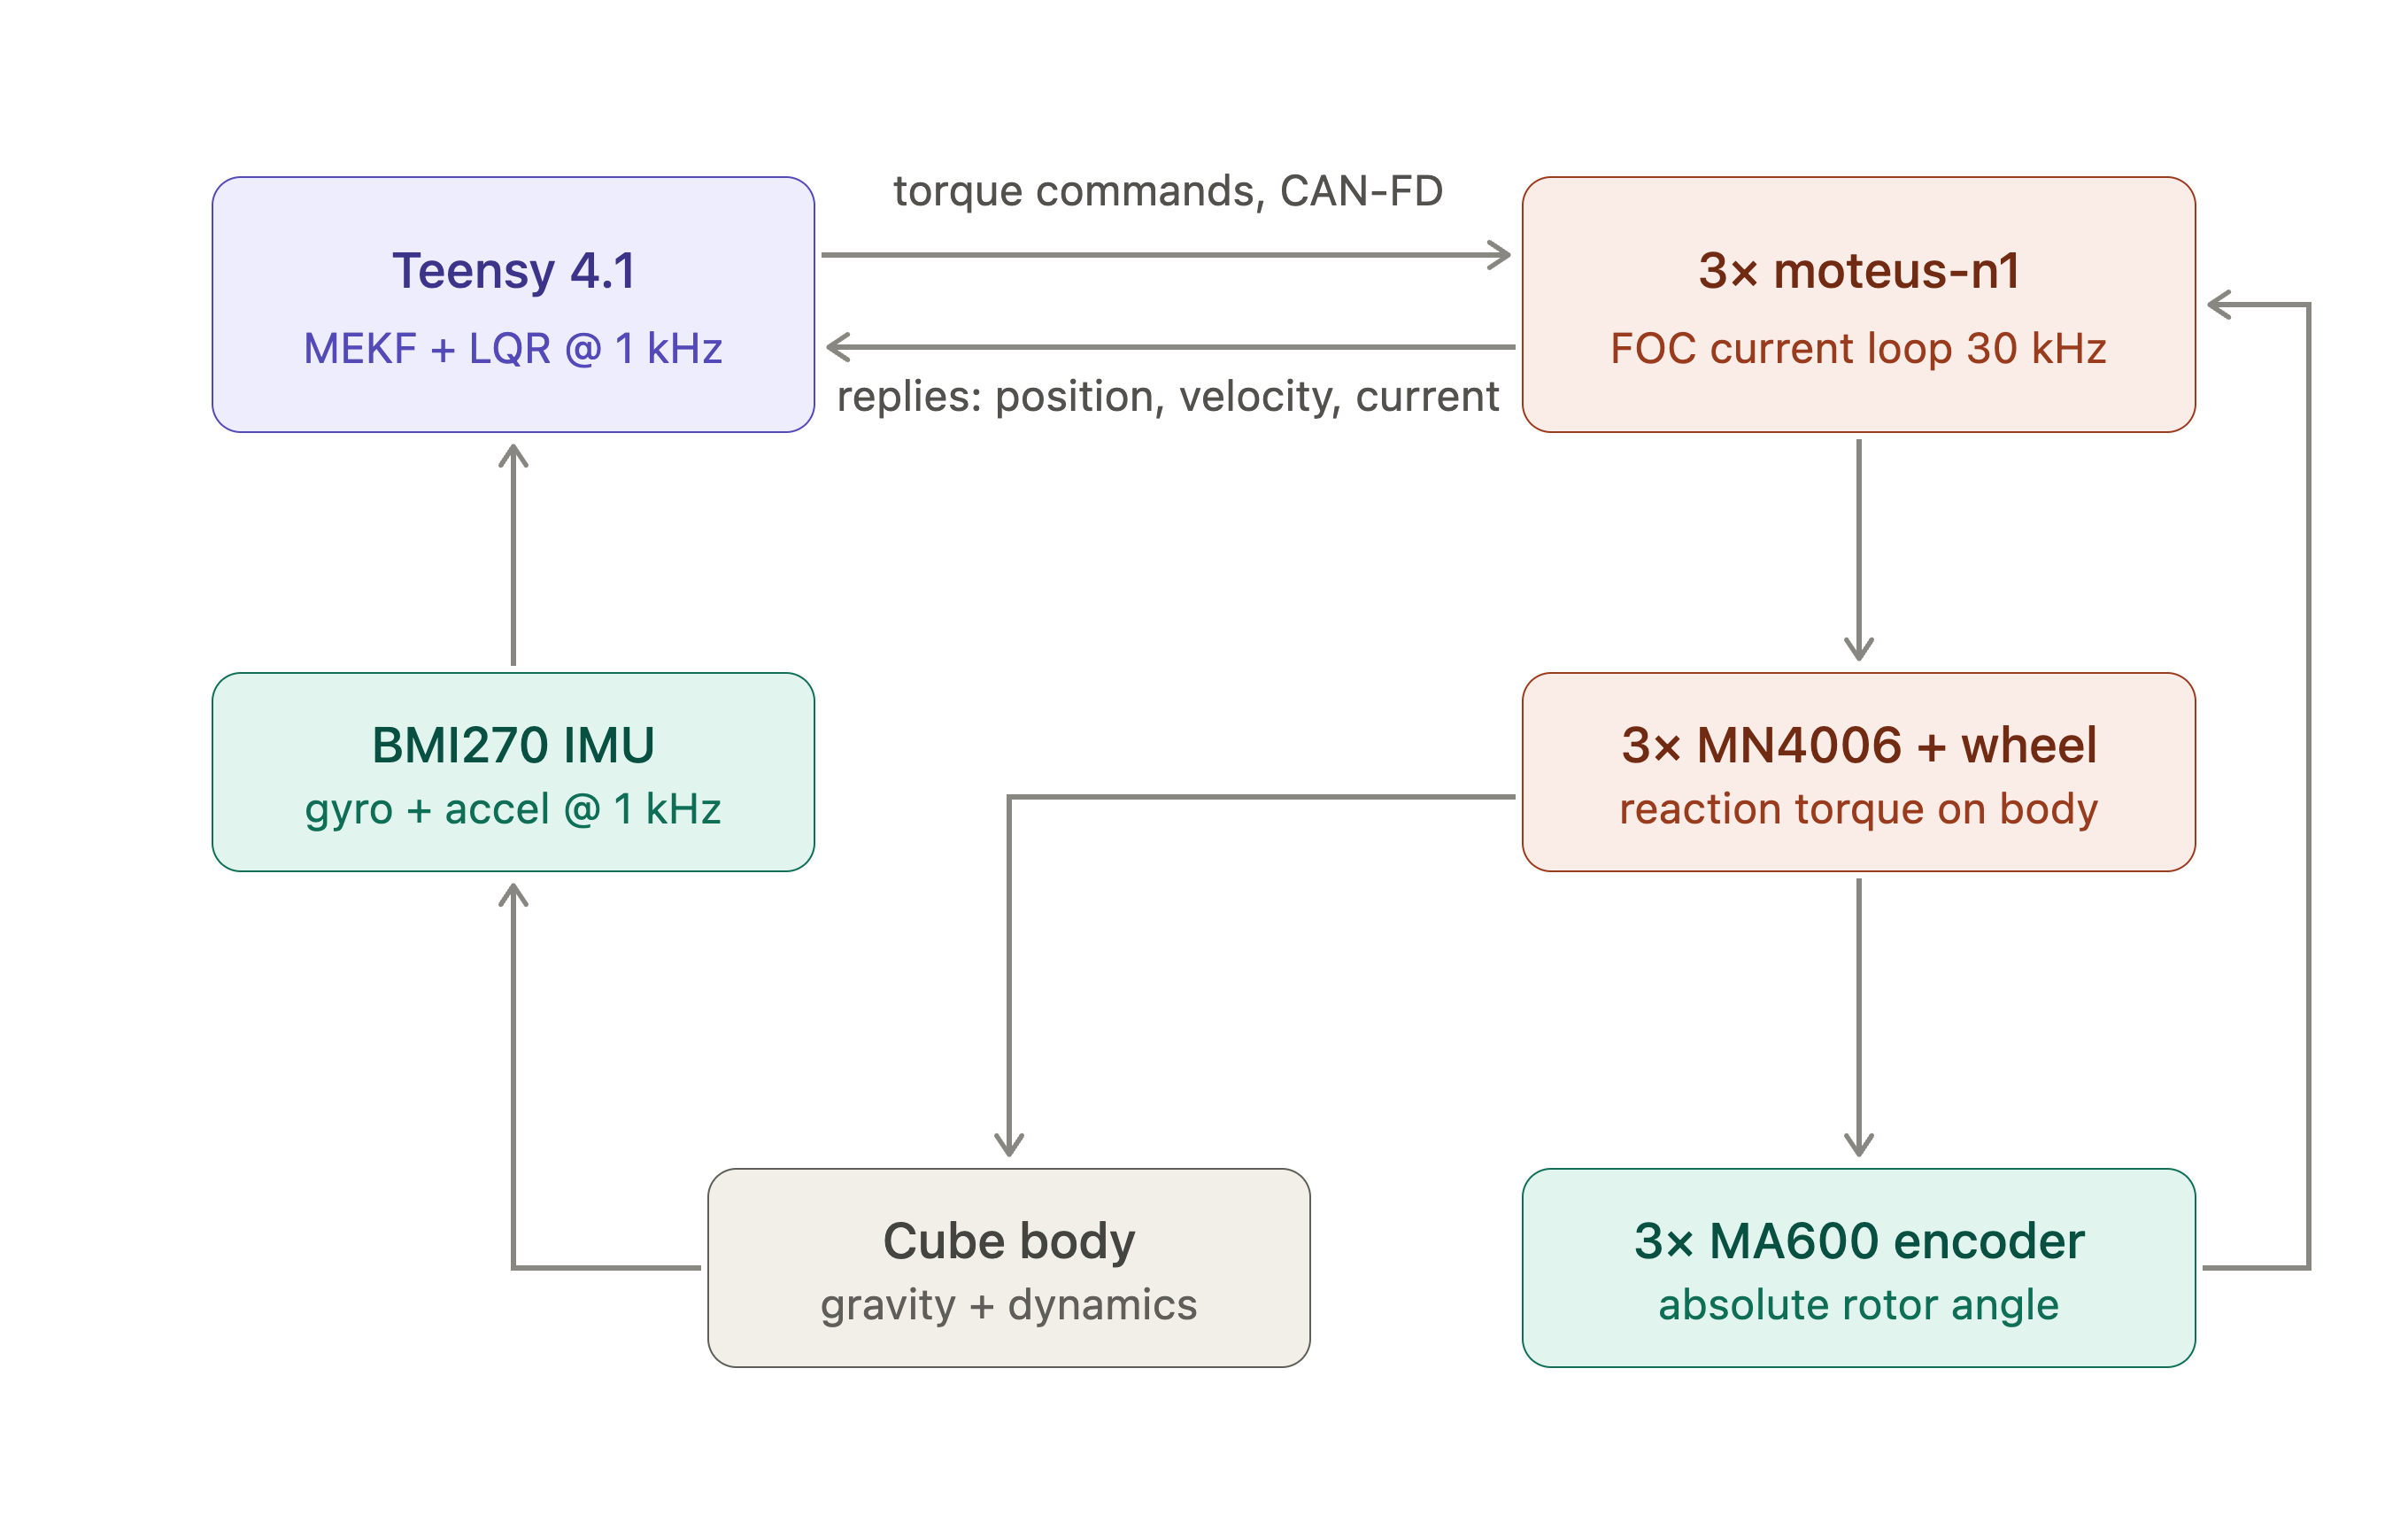
\includegraphics[width=\textwidth]{images/cubli_full_system_loop.png}
\caption[System architecture and control loop]{System architecture and control loop. Blue: processing; green: sensing;
orange: actuation. Rates shown are the design targets of
Section~\ref{sec:control_algorithms}.}
\label{fig:system_loop}
\end{figure}

\subsection{Components}

The electronics and software will be built around a microcontroller communicating over a CAN bus with a motor driver that closes the current loop for the selected brushless motor. Wheel speed will be measured with a magnetic encoder on the motor shaft, and body tilt will be estimated from an onboard IMU. Braking will be actuated by a digital servo driven directly from the microcontroller, and a wireless module will provide a telemetry and debugging link. Power will be supplied by a LiPo battery, stepped down through a DC-DC converter for the logic-level electronics, with the motor driver powered directly from the battery bus.

The full parts list is catalogued in Appendix~\ref{app:bom}
(Table~\ref{tab:bom-supplied}). The supplied set is an electronics-only BOM;
the reaction wheels, the frame and all printed parts are the team's design
responsibility, and their fabrication is the leading schedule risk.

\paragraph{Motor characterisation and operating envelope.}
Figure~\ref{fig:mn4006_curves} shows measured torque and speed against phase
current for the MN4006, taken from manufacturer bench data. The measurements
were made with the motor driving propellers rather than reaction wheels, so
the \emph{load} is not representative of this application --- an aerodynamic
load rises with the square of speed, whereas a reaction wheel is an inertia
with only bearing friction opposing it at constant speed. What does transfer
is the motor's own electromechanical behaviour, since torque per ampere and
back-EMF per unit speed are properties of the machine and not of what it is
attached to. The curves are used here only in that sense: to bound the torque
and current the actuator can be expected to deliver.

Three figures relevant to the design follow from the data. First, the
torque--current relation in Figure~\ref{fig:mn4006_curves}(a) is close to
linear ($r = 0.97$) with an incremental slope of
\qty{0.023}{\newton\metre\per\ampere} and a positive torque-axis intercept of
about \qty{0.08}{\newton\metre}. The intercept is the expected signature of
losses that do not reach the shaft --- magnetising and iron losses plus
bearing friction --- so the useful torque per ampere is the slope, and a
constant inferred by simply dividing torque by current at a single point
would overstate it (that ratio runs to \qty{0.031}{\newton\metre\per\ampere}
through the origin). Either way the motor produces at most
\qty{0.45}{\newton\metre}, an order of magnitude below the
\qty{5}{\newton\metre} brake torque assumed in
Section~\ref{sec:jumpup_target}. The two are not
alternatives: the motor stores angular momentum in the wheel over about a
second, and the brake destroys it in tens of milliseconds, so the impulsive
torque comes from the collision and not from the drive. This is why braking is
a separate mechanism rather than a motor function. Second, the highest
measured point reaches
\qty{0.45}{\newton\metre} at \qty{17.5}{\ampere}, above the
\qty{16}{\ampere} peak rating in Table~\ref{tab:bom-supplied}, and that run
terminated on the motor's thermal limit --- so the top of this envelope is a
short-duration capability, not a continuous one. Third, speeds cross the
\qty{6000}{\rpm} design ceiling of Section~\ref{sec:massbudget} only under the
lighter loads, which is consistent with that ceiling being set by bus voltage
and derating rather than by any inability of the motor to spin faster.

\begin{figure}[tbp]
\centering
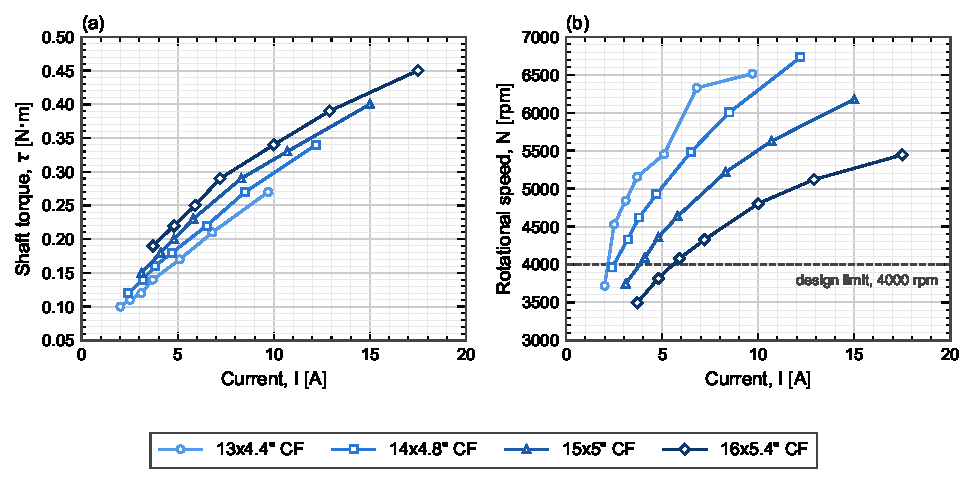
\includegraphics[width=\textwidth]{images/mn4006_torque_speed_vs_current.pdf}
\caption[Measured MN4006 shaft torque and speed against phase current]{Measured MN4006 (a) shaft torque and (b) rotational speed against
phase current, for one motor driving four different loads. Symbols are
measured points at throttle settings of 50, 55, 60, 65, 75, 85 and
\qty{100}{\percent}; lines join successive points and are not fits. The
dashed line in (b) is the \qty{6000}{\rpm} reaction-wheel design ceiling of
Section~\ref{sec:massbudget}. Loads shown are propellers, not reaction wheels:
the curves characterise the \emph{motor}, and the load-dependent spread
between them does not carry over to this application. Manufacturer static
bench data; the heaviest load reached the motor thermal limit at
\qty{100}{\percent} throttle.}%
\label{fig:mn4006_curves}%
\end{figure}

\subsection{Power Architecture}
\label{sec:power_arch}

The power architecture is shown in Figure~\ref{fig:power_tree}. A single 6S LiPo
pack (\qty{22.2}{\volt} nominal, \qty{1550}{\milli\ampere\hour}) feeds everything
through one XT60 connector, behind a combined E-stop and fuse, with an
anti-spark path to limit inrush into the driver bulk capacitance. The XT60 is
fixed by the pack rather than chosen: it is rated at
${\approx}\,\qty{60}{\ampere}$, which covers the three-axis spin-up transient
but with a smaller margin than a \qty{90}{\ampere} housing would give, so the
transient is a measured acceptance item at first power-on rather than an
assumed one. The bus
then splits into two rails. The \emph{motor bus} runs at pack voltage
(\qtyrange{22}{25}{\volt} across the discharge curve) directly into the three
moteus drivers, with bulk capacitance rated to at least \qty{50}{\volt} to absorb
regenerative braking transients---which are not incidental here, since the
jump-up manoeuvre of Section~\ref{sec:jumpup} dumps the full wheel kinetic energy
back into the bus. The \emph{logic rail} is derived by an LM2596 buck converter
stepping \qty{22}{\volt} down to \qty{5}{\volt} for the Teensy, the ESP32
telemetry link, the three brake servos and the IMU. Keeping the two rails separate
downstream of the E-stop means motor-current ripple does not reach the sensing
and processing electronics.

\begin{figure}[htbp]
\centering
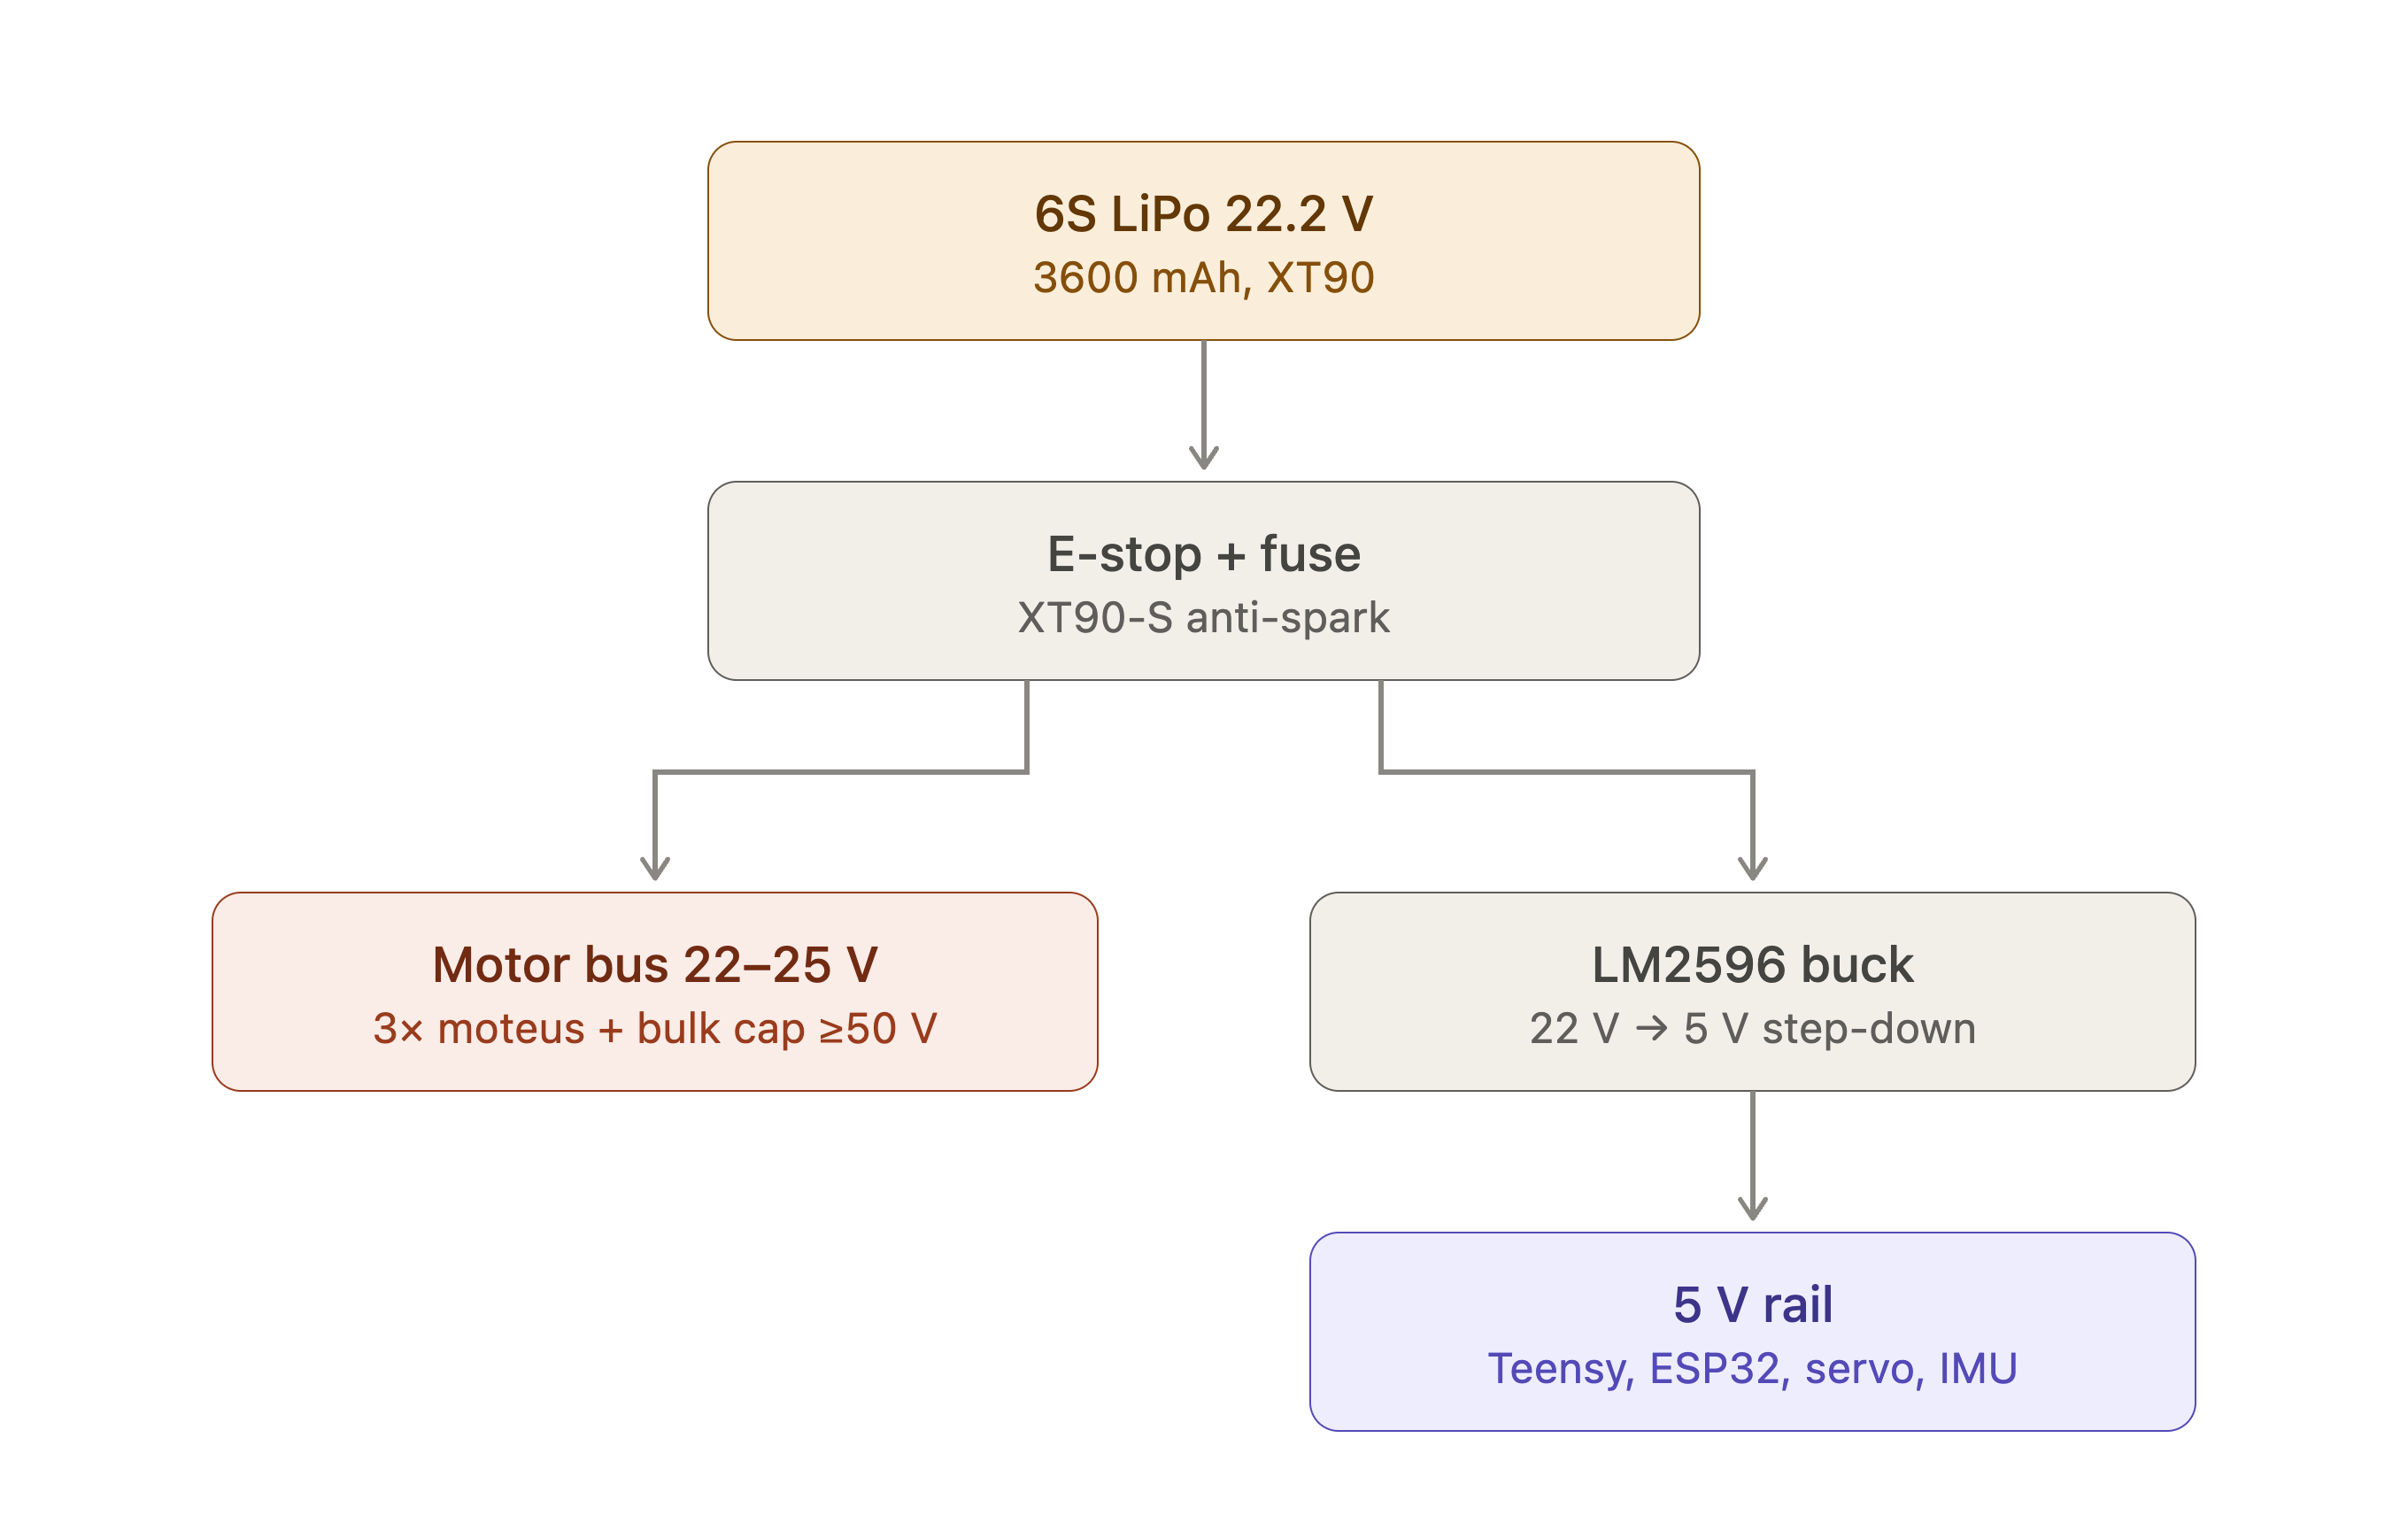
\includegraphics[width=0.9\textwidth]{images/cubli_power_tree.png}
\caption[Power distribution tree]{Power distribution tree. A single 6S pack feeds the motor bus directly
and the \qty{5}{\volt} logic rail through a buck converter, both behind a common
E-stop and fuse.}
\label{fig:power_tree}
\end{figure}

The rail-by-rail current budget that sizes the buck converter and the harness
conductors is Table~\ref{tab:power_budget}. It is populated from measurement
during bench bring-up rather than from datasheet maxima alone, because the
figure that matters for the \qty{5}{\volt} rail is the coincident worst case ---
telemetry transmit burst, servo stall and full sensor load at once --- and not
the sum of typical values.

\begin{table}[htbp]
\centering
\caption[Rail current budget]{Rail current budget. Measured values replace estimates during bench
bring-up; the \qty{5}{\volt} total is checked against the LM2596 rating, which
derates without a heatsink.}
\label{tab:power_budget}
\small
\begin{tabular}{L{4.4cm} c c c L{3.4cm}}
\toprule
Load & Rail & Typical (mA) & Worst case (mA) & Basis \\
\midrule
Teensy 4.1                & \qty{5}{\volt}  & \textcolor{red}{TBD} & \textcolor{red}{TBD} & Datasheet \\
XIAO ESP32-C6 telemetry   & \qty{5}{\volt}  & \textcolor{red}{TBD} & \textcolor{red}{TBD} & TX burst governs \\
BMI270 IMU                & \qty{5}{\volt}  & \textcolor{red}{TBD} & \textcolor{red}{TBD} & Datasheet \\
MG92B brake servos ($3\times$) & \qty{5}{\volt}  & \textcolor{red}{TBD} & \textcolor{red}{TBD} & Simultaneous stall current governs \\
MA600 encoders ($3\times$)& \qty{5}{\volt}  & \textcolor{red}{TBD} & \textcolor{red}{TBD} & Datasheet \\
\midrule
\textbf{Logic rail total} & \qty{5}{\volt}  & \textcolor{red}{\textbf{TBD}} & \textcolor{red}{\textbf{TBD}} & \textbf{vs.\ converter rating} \\
\midrule
moteus-n1 drivers ($3\times$) & Pack & \textcolor{red}{TBD} & \textcolor{red}{TBD} & Spin-up, not balance, governs \\
\bottomrule
\end{tabular}
\end{table}

\subsection{Schematic and Interconnect Diagrams}
\label{sec:schematics}

The signal-level design is documented as a set of sheets rather than a single
drawing, so that each can be checked against the constraint that governs it.
Table~\ref{tab:schematic_sheets} is the index; the sheets themselves are in
Appendix~\ref{app:schematics}, together with the connector and pin-assignment
tables. The design is currently captured as one flat schematic
(Figure~\ref{fig:schematic_full}), from which these sheets are split as each is
verified against its governing constraint; the index below is therefore the
release plan as much as it is a table of contents.

\begin{table}[htbp]
\centering
\caption[Schematic sheet index]{Schematic sheet index. Each sheet is checked against the governing
constraint stated in its row before release.}
\label{tab:schematic_sheets}
\small
\begin{tabular}{c L{4.2cm} L{7.4cm}}
\toprule
Sheet & Content & Governing constraint to verify \\
\midrule
1 & Power entry and protection & E-stop, fuse rating, anti-spark inrush into the driver bulk capacitance \\
2 & \qty{5}{\volt} logic rail & Converter rating vs.\ Table~\ref{tab:power_budget} worst case; back-feed diode; rail bulk capacitance voltage rating \\
3 & CAN-FD bus & Linear topology, stub length, split termination at the two physical ends only (Sec.~\ref{sec:bus_topology}) \\
4 & Encoder interfaces ($3\times$) & SPI cable length and encoder air gap; driver placement follows from this, not the reverse \\
5 & Flight computer and IMU & Sensor orientation and mounting location relative to the pivot (Sec.~\ref{sec:control_algorithms}) \\
6 & Telemetry link & Transmit-burst current and its return path off the logic rail \\
7 & Brake servo drive & Stall current headroom on the logic rail; PWM routing away from the encoder SPI \\
\bottomrule
\end{tabular}
\end{table}

\subsection{Bus Topology, Termination and Signal Integrity}
\label{sec:bus_topology}

The CAN-FD bus is the one electrical subsystem whose physical routing is a
correctness requirement, and it is therefore
fixed before the board outline is drawn. At the design data rate the bus must be
a linear chain with short stubs and termination at exactly the two physical
ends; a star topology or a mid-chain termination will pass a bench continuity
check and then fail intermittently under wheel vibration, which is the hardest
class of fault to diagnose once the cube is closed. The design rules and their
verification are listed in Table~\ref{tab:signal_rules}.

The encoder interfaces impose the complementary constraint. Each absolute
encoder requires a short SPI run to its own driver and a tightly held air gap to
its magnet, so the driver positions are dictated by the encoder positions, and
those in turn by the motor axes. The physical layout order is therefore: motor
axes fix the encoders, encoders fix the drivers, drivers fix the bus route, and
only then is the board outline of Section~\ref{sec:layout} drawn around what
remains.

\begin{table}[htbp]
\centering
\caption[Signal-integrity design rules and verification]{Signal-integrity design rules and how each is verified. These are
checked before cube closure, since all are hard to access afterwards.}
\label{tab:signal_rules}
\small
\begin{tabular}{L{3.4cm} L{4.6cm} L{6.0cm}}
\toprule
Interface & Rule & Verification \\
\midrule
CAN-FD bus       & Linear chain; short stubs; split termination at the two physical ends only & Differential-pair scope capture; sustained error-frame count at full rate with all nodes addressed \\
Encoder SPI      & Short run to its own driver; air gap and chip centring per the assembly spec & Read-back with no error flags; re-checked after mechanical assembly \\
IMU              & Mounted at or near the pivot; orientation per the body frame of Sec.~\ref{sec:cad_method} & Static orientation check; noise floor with wheels spinning \\
Rail separation  & Motor bus and logic rail separated downstream of the E-stop & Ripple measurement on the logic rail under motor load \\
Grounding        & Single return topology; no motor return current through the sensing ground & Continuity and isolation check before first power-on \\
\bottomrule
\end{tabular}
\end{table}

\subsection{Board Layout and Harness}
\label{sec:layout}

The electronics are built on a double-sided perfboard rather than a fabricated PCB. A PCB would have a long lead time, and a perfboard allows for iteration and modification throughout the process. Its consequence is that
layout discipline --- rail separation, decoupling at each device, deliberate
routing of the bus pair --- must be enforced by hand and checked explicitly,
since no design-rule check will do it.

The board outline, mounting-hole pattern, keep-out heights and connector exit
directions constitute the electronics-mount interface of
Table~\ref{tab:mech_interfaces} and are frozen once delivered to the mechanical
design: later electrical changes must fit inside that outline rather than move
it. The harness --- battery lead, driver drops, bus chain and servo drive ---
is fabricated to the drawings in Appendix~\ref{app:harness} and is labelled and
strain-relieved before installation, because every connector in the machine sits
on a structure that vibrates by design.

\subsection{Electrical Safety and Bring-Up Protocol}
\label{sec:electrical_safety}

Two rules govern all electrical bring-up and are stated here because they are
design constraints, not merely lab practice. First, every first-time power
application is made on a current-limited bench supply, never on the battery; the
battery is introduced only after the assembly has passed a full bench power-on.
Second, the pack is never connected without the E-stop and fuse in circuit and
the anti-spark path intact, since the driver bulk capacitance draws an inrush
that will weld a bare connector.

The staged sequence --- rails, then buses, then sensors, then open-loop motion,
then closed-loop --- and the acceptance criteria that close each step are given
with the rest of the verification work in Section~\ref{sec:verification}. The
isolation checks that precede first power-on
(rail-to-rail separation, bus-to-chassis, and confirmation that no low-voltage
capacitor sits on the pack bus) are recorded in Appendix~\ref{app:electrical}
as a checklist, because they are performed on every re-assembly and not only
once.
